\section{Introduction}

The central question addressed in this paper is: \emph{How can we produce a model that we can verify is confidence calibrated, in a sample-efficient way?}

Applications like personalized medicine, meteorological forecasting, and natural language processing require that classifiers provide calibrated confidence measures in addition to their predictions~\cite{jiang2012calibrating, brocker2009decomposition, nguyen2015posterior}.
In other words, the probability that a system outputs for an event should reflect the true frequency of that event: if an automated diagnosis system says 1,000 patient have cancer with probability 0.1, approximately 100 of them should indeed have cancer.
Most machine learning models, including neural networks, do not output calibrated probabilities out of the box~\cite{guo2017calibration, zadrozny2001calibrated}.
Instead, recalibration methods take the output of an uncalibrated model, and transform it into a calibrated probability.
Popular recalibration approaches include Platt scaling~\cite{platt1999probabilistic}, isotonic regression~\cite{zadrozny2002transforming}, and temperature scaling~\cite{guo2017calibration}. These methods are widely used, but do they actually produce calibrated probabilities?
% , and speech recognition~\cite{dong2011calibration}
% These methods use additional recalibration data to fit a simple function on top of the original model outputs.

% Important, check that it's not too similar to "On calibration of modern neural networks" paper.
% In many applications, classification models must not only be accurate, but should indicate when they may be incorrect. For example, in automated healthcare applications, control should be passed on to human doctors when the confidence of a disease diagnosis prediction is low. Specifically, classifiers should provide a \emph{calibrated} confidence measure in addition to its prediction. In other words, the probability that a system outputs for an event should reflect the true frequency of that event: of the times that a system says a patient has cancer with probability 0.3, 30\% of the time, the patient should indeed have cancer.
% Typically, complex models like neural networks do not output calibrated probabilities.
% Instead, recalibration methods take the output of an uncalibrated model, and transform it into a calibrated probability.
% Popular recalibration approaches include Platt scaling and temperature scaling.

% Recent advances in machine learning have dramatically increased predictive accuracy. Machine learning methods are now entrusted with making decisions in applications ranging from weather forecasting to medical diagnosis \pl{seems a bit naive...}. In many of these settings, classification models must not only be accurate, but should indicate when they may be incorrect. For example, in automated healthcare applications, control should be passed on to human doctors when the confidence of a disease diagnosis prediction is low. Specifically, classifiers should provide a \emph{calibrated} confidence measure in addition to its prediction. In other words, the probability that a system outputs for an event should reflect the true frequency of that event: of the times that a system says that it will rain with probability 0.3,  30\% of the time, it should rain.
% \pl{need citations; is rain prediction really driven by "modern ML"?}\tm{It also seems unncessary to introduce the rain example --- it seems to be a good introduction to people who didn't know it before, but not something to write in the first para of a paper?}

%  \pl{I'd try to combine with first paragraph so that it's all background}
% \pl{introduce calibration error as a central concern first;
% methods try to calibrate, but do they actually achieve it?
% }

\emph{We discover that these methods are less calibrated than reported.} Estimating the calibration of models can be very challenging, so past work approximates a model's calibration error using a finite set of bins. We show that by using more bins, we can uncover a higher calibration error for models on CIFAR-10 and ImageNet (Figure~\ref{fig:lower_bounds}). This is a fundamental limitation with approaches that output a continuous range of probabilities -- we show that their true calibration error may never be measurable with a finite number of bins (Example~\ref{ex:continuous-not-calibrated}).

An alternative approach, histogram binning~\cite{zadrozny2001calibrated}, outputs probabilities from a finite set.
Histogram binning can produce a model that is calibrated, and verifiably so, but it can be sample inefficient.
In particular, the number of samples required to calibrate scales linearly with the number of model outputs $B$~\cite{naeini2014binary}, which can be large particularly in the multi-class setting.
Recalibration sample efficiency is crucial -- we often want to recalibrate our models in the presence of domain shift~\cite{hendrycks2019anomaly}, and may have access to only a small labeled dataset from the target domain.

To get the sample efficiency of Platt scaling and the verification guarantees of histogram binning, \emph{we propose the variance-reduced calibrator} (Figure~\ref{fig:var_red_binning}).
As with other recalibration methods, we begin with a recalibration dataset $\{(z_1, y_1), ..., (z_n, y_n)\}$, where $z_i$ represents the uncalibrated model output and $y_i$ the ground truth label.
In the binary classification setting, $z_i \in [0, 1]$ and $y_i \in \{0, 1\}$.
We fit a simple function $g \in \mathcal{G}$ to the recalibration dataset.
We then bin the input space so that an equal number of $g(z_i)$ land in each bin.
In each bin, we output the average of the $g(z_i)$ values in that bin -- these are the gray circles in Figure~\ref{fig:var_red_binning}.
Binning ensures that the output probabilities are from a finite set, so we can check if it is calibrated.
In contrast, histogram binning takes the average of the $y_i$ values in each bin (Figure~\ref{fig:hist_binning}).
The motivation behind our method is that the $g(z_i)$ values in each bin are in a narrower range than the $y_i$ values -- when we take the average we incur less of an estimation error.
If $\mathcal{G}$ is well chosen, our method requires $O(\frac{1}{\epsilon^2})$ samples to achieve calibration error $\epsilon$ instead of $O(\frac{B}{\epsilon^2})$ samples for histogram binning, where $B$ is the number of model outputs (Theorem~\ref{thm:final-calib}).


\begin{figure}
     \centering
     \begin{subfigure}[b]{0.32\textwidth}
         \centering
         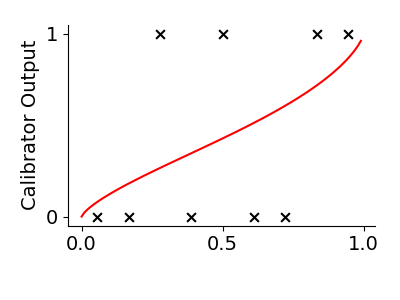
\includegraphics[width=\textwidth]{platt_scaling}
         \caption{Platt scaling.}
         \label{fig:platt_scaling}
     \end{subfigure}
     \hfill
     \begin{subfigure}[b]{0.32\textwidth}
         \centering
         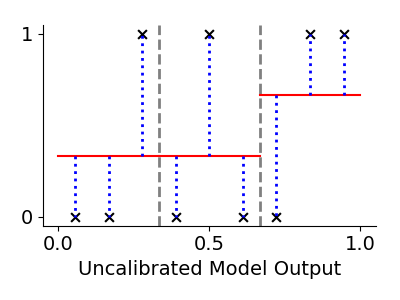
\includegraphics[width=\textwidth]{histogram_binning_with_deltas}
         \caption{Histogram binning.}
         \label{fig:hist_binning}
     \end{subfigure}
     \hfill
     \begin{subfigure}[b]{0.32\textwidth}
         \centering
         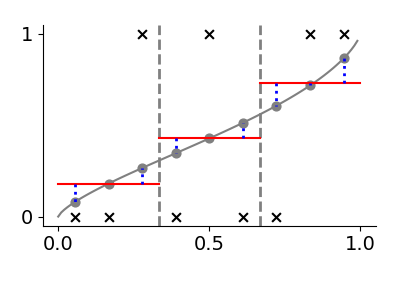
\includegraphics[width=\textwidth]{variance_reduced_binning_with_deltas}
         \caption{Variance-reduced binning.}
         \label{fig:var_red_binning}
     \end{subfigure}
        \caption{
        Visualization of the 3 recalibration approaches.
        The black crosses are the ground truth labels, and the red lines are the output of the recalibration methods.
        Platt Scaling (Figure~\ref{fig:platt_scaling}) fits a function to the recalibration data, but its calibration error is not measurable.
        Histogram binning (Figure~\ref{fig:hist_binning}) outputs the average label in each bin.
        Our variance-reduced binning (Figure~\ref{fig:var_red_binning}) fits a function $g \in \mathcal{G}$ to the recalibration data and then \emph{takes the average of the function values (the gray circles)} in each bin.
        The function values have lower variance than the labels, as visualized by the blue dotted lines, which is why our approach has lower variance. 
        }
        \label{fig:variance_reduced_illustration}
\end{figure}

Next, we turn to the important question of efficiently measuring the calibration error of a model.
Prior work~\cite{nguyen2015posterior, guo2017calibration, hendrycks2019anomaly, kuleshov2015calibrated, hendrycks2019pretraining} uses the plugin estimator for the calibration error (Definition~\ref{dfn:plugin-estimator}).
Here, again, the sample complexity of the plugin estimator scales linearly with the number of model outputs $B$.
By taking advantage of error cancellations across bins, \emph{we introduce the cancelling estimator}.
We show that the sample complexity of our estimator scales with $\sqrt{B}$ (Theorem~\ref{thm:final-ours}).

We validate our theory with multi-class calibration experiments on CIFAR-10~\cite{krizhevsky2009learningmultiple} and ImageNet~\cite{deng2009imagenet}.
The objective is to maximize the mean-squared error, also known as the Brier score~\cite{brier1950verification}, subject to a calibration constraint.
We show that the variance-reduced calibrator achieves a lower mean-squared error for any given calibration constraint.
For example, we get a \emph{2x lower mean-squared error on CIFAR-10 if we want a calibration error $\leq 3\%$.}
We also show that the canceling estimator converges to the true calibration error much faster than the plugin estimator.

